\section{Mathematical Proofs}\label{2402:sec:app:proofs}

\subsection{Notations}
We use the asymptotic notation $f_1(d)=\Theta_d(f_1(d))$ to denote $c \abs{f_1(d)} \leq \abs{f_2(d)} \leq C \abs{f_1(d)}$ for some constants $c, C > 0$ and large enough $d$. Similarly, $f_1(d)=o_d(f_1(d))$ denotes
$f_1(d) \leq c(f_1(d))$ for any constant $c > 0$ and large enough $d$.
We use $\xrightarrow[P]{d,n \rightarrow \infty}, \xrightarrow[D]{d,n \rightarrow \infty}$ to denote convergence in probability and convergence in distribution respectively as $d,n \rightarrow \infty$ with $n/d=\alpha > 0$. We denote subspaces and linear operators, matrices on  $\R^d$ through uppercase letters $A,B,C,\cdots$. For any subspace $A \in \R^d$, we denote by $A_\perp$, its orthogonal complement, i.e the subspace of vectors orthogonal to all $\vec{v} \in A$.
\subsection{DMFT and iterative conditioning}\label{2402:sec:iterative}
% \et{FIX THE TYPOS}
Unlike online SGD, the preactivations after multiple steps no longer remain Gaussian since the weights become dependent on the data. This prevents marginalizing over the orthogonal components over the preactivations and relating the learning of new directions to the Hermite decomposition of the target function.
Our proof circumvents these issues by utilizing a simpler effective process that decouples the pre-activations for different samples. The effective process is obtained using a rigorous version of the Dynamical Mean Field Theory derived in \citep{montanari2022universality} and \citep{gerbelot2022rigorous}.

The derivation of Dynamical Mean Field Theory in the above works has the following essential elements:

\begin{itemize}
    \item[1.] Iterative conditioning: The proof in  \citep{gerbelot2022rigorous,montanari2022universality} for obtaining the DMFT equations relies on the observation that the gradient descent algorithm in Equation \eqref{2402:eq:act_update} for a finite-number of iterations can be described completely through projections of the inputs design matrix $\vec{Z} \in \R^{n \times d}$ along a finite number of vectors in $\R^n, \R^d$. The iterative conditioning technique \citep{bolthausen2014iterative,bayati2011dynamics} then involves replacing the components of $\vec{Z} \in \R^{n \times d}$ along directions orthogonal to these projections by independent Gaussian random variables. This leads to a non-Markovian structure in the effective processes for the activations, parameters. 
     \item[2.] The concentration of finite-dimensional order parameters such as overlaps of the neuron parameters with the teacher neurons/subspace as well as expectations w.r.t the empirical measure of the pre-activations and parameters. 
\end{itemize}

Using the above elements, DMFT provides a low-dimensional effective dynamics characterizing the limiting joint empirical measure of the student parameters, as well as the pre-activations. 
We illustrate the proof for the activations after the first gradient step, illustrating the relationship with the ``hidden progress" described in section \ref{2402:sec:hidden_prog}


Let $\vec{H}^{(t)} = \frac{1}{\sqrt{d}}\vec{Z}(\vec{W}^{(t)})^\top$ denote the $n \times p$ matrix of pre-activations at time $t$. Similarly, let $\vec{H}^* \in \R^{n\times k}$ denote the matrix of input activations in the target function. We denote by $\nabla_{\vec{H}} \mathcal{L}(\vec{H}^{*},\vec{H}^{(t)}) \in \R^{n \times p}$, the matrix derivative of $\mathcal{L}$ w.r.t the corresponding entries of the pre-activations matrix $\vec{H}^{(t)}$.
After each gradient update, $\vec{W}^{(t)}$ and the preactivations $\vec{H}^{(t)}$ gain a dependence on $\vec{Z}$.
 The Iterative conditioning technique works around this dependence by 
 conditioning on the sigma algebra generated by $\vec{H}^{(t)},\vec{H}^*$ and $\vec{W}^{(t)}$ instead of on $\vec{Z}$.
 Since $\vec{Z}$ interacts with $\vec{W}^{(t)}$ and 
$\vec{H}^{(t)}$ only through projections (along right with $\vec{W}^{(t)}$ and left with $\nabla_{\vec{H}} \mathcal{L}(\vec{H}^{*},\vec{H}^{(t)})$ respectively), the conditioning allows the components of $\vec{Z}$ orthogonal to $\nabla_H \mathcal{L}(\vec{H}^{(*)},\vec{H}^{(t)})$ and $\vec{W}^{(t)}$ to be replaced by independent Gaussian entries.  

For the first-gradient step, we only require conditioning on $\vec{H}^{(0)}, \vec{H}^{*}, \vec{W}^{0}$.

From (\eqref{2402:eq:GD_update}), we obtain the following update for $\vec{H}^{(1)}$:
\begin{equation}\label{2402:eq:act_update}
    \vec{H}^{(1)}= \vec{H}^{(0)} + \frac{\eta}{d}\vec{Z}(\vec{Z})^\top  \nabla_{\vec{H}} \mathcal{L}(\vec{H}^*, \vec{H}^{(0)})\vec{a}^\top,
\end{equation}
Let $\vec{\bar{W}}^{(0)} = \begin{pmatrix}
    \vec{W}^{(0)}\\
    \vec{W}^{\star}
\end{pmatrix} \in \R^{p+k \times d}$
By the equivalence of projection and conditioning for Gaussian random variables, we have that the following inequality holds in distribution:
\begin{equation}
\vec{Z}\vert_{\vec{H}^{0},\vec{H}^*,\vec{\bar{W}}^{(0)}} \overset{d}{=} \vec{Z}P_w^\top + \tilde{\vec{Z}}(P^{\perp}_w)^\top,
\end{equation}
where $\tilde{\vec{Z}}$ is independent of $\vec{Z}$ and $P_w$ denote the projection operator along $\vec{\bar{W}}^{(0)},\vec{\bar{W}}^{\star}$, defined as:
\begin{align*}
    P_w = \vec{\bar{W}}^{(0)} (\vec{\bar{W}}^{(0)}(\vec{\bar{W}}^{(0)})^\top)^{-1}(\vec{\bar{W}}^{(0)})^\top. 
\end{align*}


Substituting in Equation (\eqref{2402:eq:act_update}), we obtain:
\begin{equation}\label{2402:eq:act_iterative}
    \vec{H}^{(1)} \overset{d}{=} \vec{H}^{(0)} +
    \eta \frac{1}{d}\tilde{\vec{Z}}(P^{\perp}_w)^\top P^{\perp}_w(\tilde{\vec{Z}})^\top \nabla_{\vec{H}} \mathcal{L}(\vec{H}^*, \vec{H}^{(0)})\vec{a}^\top + \eta\frac{1}{d}\vec{H_0}(\vec{\bar{W}}^{(0)}(\vec{\bar{W}}^{(0)})^\top)^{-1}(\vec{H_0})^\top \nabla_{\vec{H}} \mathcal{L}(\vec{H}^*, \vec{H}^{(0)})\vec{a}^\top
\end{equation}
Since the projection, $P_w$ is along a low-dimensional subspace of dimension at most $p$, we have $P^{\perp}_w \approx \mathbf{I}_d$. 
One can therefore show that $\frac{1}{\sqrt{d}}\tilde{\vec{Z}}(P^{\perp}_w)^\top P^{\perp}_w(\tilde{\vec{Z}})^\top \vec{u}$ converges in probability to $\tilde{\vec{Z}} \tilde{\vec{Z}}^\top \vec{u}$. for any deterministic $\vec{u} \in \R^d$ with $\norm{u}= \cO(\sqrt{d})$. Applying it to the vector $\vec{u} = \mathcal{L}(\vec{H}^*, \vec{H}^{(0)})$, conditioned on $\vec{H}^*, \vec{H}^{(0)}$, we obtain that:
\begin{equation}
 \frac{1}{\sqrt{d}}\norm{\frac{1}{d}\tilde{\vec{Z}}(P^{\perp}_w)^\top P^{\perp}_w(\tilde{\vec{Z}})^\top \nabla_{\vec{H}} \mathcal{L}(\vec{H}^*, \vec{H}^{(0)}) - \frac{1}{d}\tilde{\vec{Z}}(\tilde{\vec{Z}})^\top \nabla_{\vec{H}}\mathcal{L}(\vec{H}^*, \vec{H}^{(0)})}_F    \xrightarrow[P]{n,d \rightarrow \infty} 0. 
\end{equation}
Now, the diagonal entries of $\frac{1}{d}\tilde{\vec{Z}}(\tilde{\vec{Z}})^\top$ convergence in probability to $1$ due to the concentration of norms of Gaussian random vectors. This results in the term $\mathcal{L}(\vec{H}^*, \vec{H}^{(0)})$. This term is precisely the one responsible for the ``hidden progress" explained in section \ref{2402:sec:hidden_prog}, corresponding to the term in Equation \ref{2402:eq:hid_prog_term}. Since $\tilde{\vec{Z}}$ is independent of $\vec{W}^{(0)}$ and $\vec{H}^{(0)}, \vec{H}^*$, by central limit-theorem for sub-Gaussian random variables, the remaining off-diagonal terms can be shown to converge to Gaussian noise independent of $\vec{H}^{(0)}, \vec{H}^*$ with variance $\norm{\nabla_{\vec{h}} \mathcal{L}(\vec{h}^*, \vec{h}^{(0)})}^2$. 

Lastly, the third term in Equation \eqref{2402:eq:act_iterative} can be shown to converge to Gaussian noise correlated with corresponding entries of $\vec{H_0},\vec{H^*}$.
Specifically, by removing the conditioning on $\vec{H_0}$, we have through law of large numbers and Stein's Lemma, we have that the term $\frac{1}{d}(\vec{H_0})^\top \nabla_{\vec{H}} \mathcal{L}(\vec{H}^*, \vec{H}^{(0)})$ converges in probability to $(\vec{W}^{(0)}(\vec{W}^{(0)})^\top) \Ea{\nabla^2_{\vec{h}}\mathcal{L}(\vec{h}^*, \vec{h}^{(0)})}$. Therefore, we obtain:
\begin{equation}
    \frac{1}{\sqrt{d}}\norm{\frac{1}{d}\vec{H_0}(\vec{W}^{(0)}(\vec{W}^{(0)})^\top)^{-1}(\vec{H_0})^\top \nabla_{\vec{H}} \mathcal{L}(\vec{H}^*, \vec{h}^{(0)})\vec{a}^\top - \vec{H_0}\Ea{\nabla^2_{\vec{h}}\mathcal{L}(\vec{h}^*, \vec{h}^{(0)})})\vec{a}^\top} \xrightarrow[P]{n,d \rightarrow \infty} 0
\end{equation}


Proceeding similarly, one obtains low-dimensional effective processes for $\vec{W}^{(t)},\vec{H}^{(t)}$ for any time $t \in \N$.  In the following section, we derive the resulting DMFT dynamics for the setup considered in Section \ref{2402:sec:main:introduction} through a reduction to the result in \citep{gerbelot2022rigorous}. We refer to \citep{gerbelot2022rigorous,celentano2021high} for detailed proofs based on the above technique.



% In particular, one can show that the components of the pre-activations orthogonal to the ``learned directions", denoted here by $\boldsymbol{r}_\perp$ can be replaced by independent samples from the following low-dimensional dynamics:

% \begin{equation}\label{2402:eq:rec}
% \boldsymbol{r}^{\tau+1}_\perp -  \boldsymbol{r}^\tau_\perp= -\alpha \eta\boldsymbol{r}^\tau_\perp \Lambda^\tau - \eta\nabla_{\boldsymbol{r}} \mathcal{L}(\boldsymbol{r}^{(t)}, \boldsymbol{r}^*) - \alpha\eta \sum_{t=0}^{\tau-1} \boldsymbol{r}^{(t)}_\perp R_\ell(\tau,t) + \sqrt{\alpha}\eta \boldsymbol{u}^\tau
% \end{equation}
% We observe that $\boldsymbol{r}^{1}_\perp$ depends on $\boldsymbol{r}^*$

% Next, we consider the projection of the gradient w.r.t a new direction $\langle \bz, \vec{v} \rangle$.
% \begin{equation}
%     \mathbb{E}[y\sigma'(\langle \bz,\vec{w}^{(t)}_j\rangle)\langle \bz, \vec{v} \rangle]
% \end{equation}
% For any $v$ in the teacher subspace, $\boldsymbol{r}^{t}_\perp$ depends on $\langle \bz, \vec{v} \rangle$. However, for directions having only even components in the target function, $\boldsymbol{r}^{t}_\perp$ remains an even function.
% Taking expectations w.r.t Gaussian random variables $\langle \bz, \vec{v} \rangle$ and $r^*=M^{(t)}W^*\bz$, we observe that the overlap is non-zero for directions with odd terms in the target function and activation functions having even terms in the Hermite expansion of $\sigma'$.

\subsection{Derivation of the exact asymptotics}



We start by stating a general consequence of the main result in \citep{gerbelot2022rigorous}.

\begin{theorem}[Corollary of Theorem 3.2 in \citep{gerbelot2022rigorous}]
\label{2402:thm:Cedric_theorem}
Let $W^{0} \in \R^{q \times d}$ be a sequence of matrices such that the overlap matrix satifies:
\begin{equation}
    \frac{1}{d}W^{0}(W^{0})^\top \xrightarrow[a.s]{d \rightarrow \infty} Q^{(0)},
\end{equation}
where $Q^{(0)} \in \mathcal{S}^+_p$ denotes
a fixed matrix.  Consider a dynamics of the form:
    \begin{align}
        W^{(t+1)} =  W^{(t)} - \eta \lambda W^{(t)} - \eta \frac{1}{\sqrt{d}}\sum_{\nu=1}^n F\left(\frac{ W^{(t)}\vec z_\nu} {\sqrt{d}}\right) \vec z_\nu^\top
    \end{align}
where $F:\R^q \rightarrow \R^q$ is pseudo-Lipshitz of finite-order and $\{z_\nu\}_{\nu =1}^n $ are i.i.d vectors distributed as $z_\nu \sim \mathcal{N}(0, \mathbb{I}_d)$, such that $n,d \rightarrow \infty$ with $n/d =\alpha >0$.
    % \begin{align}
    %         \label{2402:eq:the_dynamics1}
    %         \mathbf{v}^{t+1} &= \mathbf{f}_1^{t}\left(\left\{\mathbf{v}^{k}\right\}_{k=0}^{t}\right)+\mathbf{Z}^{\top}\mathbf{f}_2^{t}(\mathbf{r}^{t})  \\
    %         \mathbf{r}^{t} &= \mathbf{Z}\sum_{k=0}^{t}\mathbf{v}^{k} .
    %         \label{2402:eq:the_dynamics2}
    %     \end{align},
    % where $\mathbf{Z}$ is an $n \times d$ matrix with i.i.d Gaussian entries and $f_1,f_2,\mathbf{v}$ satisfy assumptions A1-A7 in \citep{gerbelot2022rigorous}.
    Then the empirical measure of the weights $ \vec w^{(t)}_i$ converges in distribution to the weight process $\vec \theta_i^{(t)}$ and the  empirical measure of the preactivations $\vec h^{(t)}_\nu$ converges in distribution to that of the  preactivation process $\vec h^{(t)}$, defined as    
    \begin{equation}\label{2402:eq:proc_theta}
        \boldsymbol{\theta}^{(t+1)} -  \boldsymbol{\theta}^{(t)}= - \eta \left(\lambda + \Lambda^{(t)}\right)\boldsymbol{\theta}^{(t)} +\eta \sum_{\tau=0}^{t-1}  R_\ell^{(t,\tau)} \boldsymbol{\theta}^{(\tau)} + \eta \boldsymbol{u}^{(t)}
    \end{equation}
    \begin{equation}\label{2402:eq:proc_h}
        \boldsymbol{h}^{(t)} = -\eta\sum_{\tau=0}^{t-1} R_\theta^{(t,\tau)} F(\boldsymbol{h}^{(\tau)}) + \boldsymbol{\omega}^{(t)}
    \end{equation}
    were we have
    \begin{equation}
        \Lambda^{(t)} = \alpha\mathbb{E}\left[ \nabla_{\boldsymbol{h}} F (\boldsymbol{h}^{(t)})\right]
    \end{equation}
    \begin{align} 
        R_\theta^{(t,\tau)} = \mathbb{E}\left[\frac{\partial \vec \theta^{(t)}}{\partial \vec \tau^{(\tau)}} \right]
    \end{align}
    \begin{align}
        R_\ell^{(t,\tau)} = \alpha \mathbb{E}\left[\frac{\partial F(\vec h^{(t)})}{\partial \vec\omega^{(\tau)}} \right].
    \end{align}
    Finally, $\boldsymbol{u}^{(t)}$ and $\boldsymbol{\omega}^{(t)}$ are zero-mean Gaussian processes respectively with covariances given by $C_\ell^{(t,\tau)}$ and $C_\theta^{(t,\tau)}$:
    
    \begin{equation}
        C_\ell^{(t, \tau)} = \alpha\mathbb{E}\left[ \boldsymbol{u}^{(t)}\left(\boldsymbol{u}^{(\tau)}\right)^\top \right] = \alpha \mathbb{E}\left[ F(\boldsymbol{r}^{(t)})F (\boldsymbol{r}^{(\tau)})^\top\right]
    \end{equation}
    \begin{equation}
        C_\theta^{(t, \tau)} = \mathbb{E}\left[\boldsymbol{\omega}^{(t)}\left(\boldsymbol{\omega}^{(\tau)} \right)^\top\right] = \mathbb{E}\left[ \boldsymbol{\theta}^{(t)}\left(\boldsymbol{\theta}^{(\tau)}\right)^\top \right]
    \end{equation}

The convergence in distribution of the empirical measures holds in the following sense:
    For any $t \in \mathbb{N}$, and any 
        pseudo-Lipschitz functions $\psi: \mathbb{R}^{p(t+1)} \to \mathbb{R}$ and $\phi: \mathbb{R}^{pt} \to \mathbb{R}$:
        \begin{align}
            &\frac{1}{d}\sum_{i=1}^{d}\psi((W_{i}^{(0)}, ..., W_{i}^{(t)})) \xrightarrow[n,d \to 
            \infty]{\whp} \mathbb{E}\left[\psi(\boldsymbol{\theta}^{(0)}, ...,\boldsymbol{\theta}^{(t)})\right], \\ &\frac{1}{n}\sum_{\nu=1}^{n}\phi((\mathbf{h}_\nu^{(0)}, ..., \mathbf{h}_{\nu}^{(t-1)})) \xrightarrow[n,d \to \infty]{\whp} \mathbb{E}\left[\phi(\vec{h}^{(0)}, ..., \vec{h}^{(t-1)})\right],
        \end{align}
where $W_{i}^{(t)}$ denotes the $i_{th}$ column of $W^{(t)}$
\end{theorem}
The above result follows directly by substituting $\frac{1}{\sqrt{d}} \vec{Z}$ as $\vec{X}$ in Theorem 3.2 of \cite{gerbelot2022rigorous}.

The definitions of $R_\theta$ and $R_\ell$ in Theorem \ref{2402:thm:Cedric_theorem} require differentiating through the non-markovian processes defined by Equations \ref{2402:eq:proc_h}, \ref{2402:eq:proc_theta}. Fortunately,  $R_\theta, R_\ell$ can be equivalently described through an explicit set of recursive updates, which we state below for convenience:
    \begin{equation}
        R_\theta^{(t+1, \tau)} - R_\theta^{(t, \tau)} = - \eta \left(\lambda + \Lambda^{(t)}\right)R_\theta^{(t, \tau)} +\eta \sum_{s=\tau}^{t-1}  R_\ell^{(t,s)} R_\theta^{(\tau, s)} 
    \end{equation}
    with boundary conditions
    \begin{align}
        &R_\theta^{(t, t)} = 1, \\
        &R_\theta^{(t+1, t)} = 1 - \eta \Lambda^{(t)},
    \end{align}
while 
\begin{equation}
    R_\ell^{(t, \tau)} = \alpha\mathbb{E}\left[\nabla_{\boldsymbol{h}} F (\boldsymbol{h}^{(t)}) T_\ell^{(t, \tau)} \right],
\end{equation}
where $T_\ell^{(t, \tau)}$ is a collection of stochastic processes with distribution 
\begin{equation}
    T_\ell^{(t, \tau)} = R_\theta^{(t,\tau)}\nabla_{\boldsymbol{h}} F (\boldsymbol{h}^{(\tau)}) + \sum_{s=\tau+1}^{t-1} R_\theta^{(t,s)}  T_\ell^{(s, \tau)} 
\end{equation}
and boundary conditions
\begin{align}
    &T_\ell^{(t, t)} = 0, \\
    &T_\ell^{(t+1, t)} = 1 - \eta \Lambda^{(t)},
\end{align}

    
To obtain the limiting equations under the setting of gradient descent with teacher weights $W^*$ in section \ref{2402:sec:main:introduction}, we utilize the generality of the update $F$ in theorem \ref{2402:thm:Cedric_theorem}, which allows for a portion of the parameters ($W^*$) to remain unaffected. We obtain the following result, which generalize the former theorem to the setting of our paper:
\begin{theorem}\label{2402:thm:DMFT_committee}
Consider the distribution over data defined in section \ref{2402:sec:main:setting} and an update rule on the weights of the form \eqref{2402:eq:GD_update}, i.e:
    \begin{align} 
    \vec w_i^{(t+1)} = \vec w^{(t)}_i - \eta \lambda \vec w^{(t)}_i - \eta \sum_{\nu=1}^n\nabla_{\vec w^{(t)}_i} \mathcal{L}\left(\frac{W^{(t)}\vec z_\nu} {\sqrt{d}}, \frac{W^\star\vec z_\nu} {\sqrt{d}} \right),
    \end{align}
Then under the assumptions of Theorem \ref{2402:thm:main:2step_learning}, as $d \rightarrow \infty$ with $n/d=\alpha >0$, the joint empirical measure of the coordinates of the student weights $\vec w_i^{(t)}$ and the teacher weights
$W^\star$  converges in distribution to  the stochastic process $\vec{\theta}^{(t)}$ and the standard normal variable $\vec{\theta^\star}$, in the sense of Theorem \ref{2402:thm:Cedric_theorem}. Similarly, the joint empirical measure of the student and teacher preactivations $\frac{\vec w_i^{(t)}\vec z_\nu} {\sqrt{d}}$, $\frac{\vec w_i^\star\vec z_\nu} {\sqrt{d}}$ converge in distribution to the stochastic process
$\vec{h}^{(t)}$ and the standard normal variable $\vec{h}^\star$. $\boldsymbol{\theta}^{(t)}$ and $\vec{h}^{(t)}$ are defined recursively through the following equations:
\begin{equation} \label{2402:eq:def_theta_planted}
    \boldsymbol{\theta}^{(t+1)} -  \boldsymbol{\theta}^{(t)}= - \eta\left(\lambda + \Lambda^{(t)}\right)\boldsymbol{\theta}^{(t)} +\eta \sum_{\tau=0}^{t-1}  R_\ell^{(t,\tau)}\boldsymbol{\theta}^{(\tau)} - \eta g^{(t)}\boldsymbol{\theta}^\star + \eta \sum_{\tau=0}^{t}  \tilde R_\ell^{(t,\tau)}\boldsymbol{\theta}^\star + \eta \boldsymbol{u}^{(t)}
\end{equation}
\begin{equation} \label{2402:eq:def_h_planted}
    \boldsymbol{h}^{(t)} = -\eta\sum_{\tau=0}^{t-1}R_\theta^{(t,\tau)} \nabla_{\boldsymbol{h}} \ell(\boldsymbol{h}^{(\tau)}, \boldsymbol{h}^\star) + \boldsymbol{\omega}^{(t)}
\end{equation}
% where we $\Lambda^{(t)}$, $R_\ell^{(t, \tau)}$ and $R_\theta^{(t, \tau)}$ are defined as in \ref{2402:thm:Cedric_theorem}. 
Here $\vec u^{(t)}, \boldsymbol \theta^\star$ and $(\boldsymbol \omega^{(t)},  \boldsymbol h^\star)$ are zero mean Gaussian Process with covariances $C_\ell^{(t,\tau)}$ and $\Omega^{(t,\tau)}$ respectively, given by:
\begin{align} 
    C_\ell^{(t, \tau)} =   \alpha\mathbb{E}\left[ \boldsymbol{u}^{(t)}\left(\boldsymbol{u}^{(\tau)}\right)^\top \right] =
    \alpha \mathbb{E}_{\boldsymbol{h}^{(t)}, \boldsymbol{h}^\star}\left[ \nabla_{\boldsymbol{h}} \mathcal{L}(\boldsymbol{h}^{(t)}, \boldsymbol{h}^\star)\nabla_{\boldsymbol{h}} \mathcal{L}(\boldsymbol{h}^{(\tau)}, \boldsymbol{h}^\star)^\top\right] \label{2402:eq:def_C_l} \\
    \Omega^{(t,\tau)} =   \mathbb{E}\left[ \begin{pmatrix}
       \boldsymbol \omega^{(t)} \\   \boldsymbol h^\star
    \end{pmatrix} \begin{pmatrix}
        \boldsymbol \omega^{(t)}   \\ \boldsymbol h^\star 
    \end{pmatrix}^\top \right]= \begin{bmatrix}
        C_\theta^{(t,\tau)} & M^{(t)} \\
        M^{(t)} & 1
    \end{bmatrix}\label{2402:eq:def_C_omega},
\end{align}
where $C_\theta^{(t,\tau)}, M^{(t)}$ are defined as:
\begin{align}
\begin{bmatrix}
        C_\theta^{(t,\tau)} & M^{(t)} \\
        M^{(t)} & 1
    \end{bmatrix} =  \mathbb{E}_{\boldsymbol{\theta}^{(t)}, \boldsymbol{\theta}^\star}\left[ \begin{pmatrix}
        \boldsymbol{\theta}^{(t)} \\  \boldsymbol{\theta}^\star
    \end{pmatrix} \begin{pmatrix}
        \boldsymbol{\theta}^{(\tau)}   \\ \boldsymbol{\theta}^\star 
    \end{pmatrix}^\top \right]
\end{align}
The effective regularisation $\Lambda^{(t)}$ and the projected gradient $g^{(t)}$ concentrate to
\begin{align}
    \Lambda^{(t)} = \alpha\mathbb{E}_{\boldsymbol{h}^{(t)}, \boldsymbol{h}^\star}\left[\nabla^2_{\vec h}\mathcal{L}\left( \vec h^{(t)}, \boldsymbol{h}^\star\right)\right],\\ g^{(t)}=\alpha \mathbb{E}_{\boldsymbol{h}^{(t)}, \boldsymbol{h}^\star}\left[\nabla_{\vec h}\mathcal{L}\left( \vec h^{(t)}, \boldsymbol{h}^\star\right) \vec h^{\star\top}\right]
\end{align}
The memory kernels $R_\ell^{(t,\tau)}$, $\tilde R_\ell^{(t,\tau)}$, $R_\theta^{(t,\tau)}$ for $t > \tau$ are defined through the partial derivatives with respect to the noise:
\begin{eqnarray}
    &R_\theta^{(t,\tau)} = \mathbb{E}_{\boldsymbol{\theta}^{(t)}, \boldsymbol{\theta}^\star}\left[\frac{\partial \vec \theta^{(t)}}{\partial \vec \tau^{(\tau)}} \right], \nonumber  \\
    &R_\ell^{(t,\tau)} = \alpha \mathbb{E}_{\boldsymbol{h}^{(t)}, \boldsymbol{h}^\star}\left[\frac{\partial \nabla_{\vec h}\mathcal{L}\left( \vec h^{(t)}, \boldsymbol{h}^\star\right)}{\partial \boldsymbol\omega^{(\tau)}} \right],\\
    &\tilde R_\ell^{(t,\tau)} = \alpha \mathbb{E}_{\boldsymbol{h}^{(t)}, \boldsymbol{h}^\star}\left[\frac{\partial \nabla_{\vec h}\mathcal{L}\left( \vec h^{(t)}, \boldsymbol{h}^\star\right)}{\partial \left(\boldsymbol\omega^\star\right)^{(\tau)}} \right],\quad
\end{eqnarray}
and $R_\ell^{(t,t)} = \tilde R_\ell^{(t,t)} = 0$, $R_\theta^{(t,t)}=1$.
% The new memory kernel is $\tilde R_\ell^{(t,\tau)}$ is:
% \begin{align}
%     \tilde R_\ell^{(t,\tau)} = \alpha \mathbb{E}_{}\left[\frac{\partial \nabla_{\boldsymbol{h}} \ell(\boldsymbol{h}^{(t)}, \boldsymbol{h}^\star)}{\partial \left(\vec\omega^\star\right)^{(\tau)}} \right].
% \end{align}
Finally, $M^{(t)}$ satisfies the update equation    
\begin{equation} \label{2402:eq:def_M_rec}
    M^{(t+1)} =(1-\eta\lambda) M^{(t)} -\eta g^{(t)},
\end{equation}
where $g^{(t)}$ is defined as:
\begin{equation}\label{2402:eq:def_gt}
    \alpha \mathbb{E}\left[ \nabla_{\boldsymbol{h}} \ell(\boldsymbol{h}^{(t)}) \left( \boldsymbol{h}^* \right)^\top\right]
\end{equation}
\end{theorem}

\begin{proof}
  Analogous to the embedding of planted vectors in \citep{celentano2021high}, we start by considering an a lifted dynamics defined by concating $W^{(t)}$ and $W^*$. First, define the extended parameters ${\tilde W}^{(t)}\in \mathbb{R}^{(p+k)\times d}$ with update rule:
    
    \begin{align} \label{2402:eq:combined_GD}
        \begin{bmatrix} W^{(t+1)} \\ W^* \end{bmatrix} = \begin{bmatrix} W^{(t)} \\ W^* \end{bmatrix} -\eta \begin{bmatrix} \lambda W^{(t)} \\ 0 \end{bmatrix} - \eta \sum_{\nu=1}^n\begin{bmatrix}
            \nabla_{W^{(t)}} \mathcal{L}\left(\frac{W^{(t)}\vec z^\nu} {\sqrt{d}}\right) \\0
        \end{bmatrix},
    \end{align}
   The above form of updates can be seen to be a special case of Theorem \ref{2402:thm:Cedric_theorem} with $q=p+k$ and $F: R^{p+k} \rightarrow \R^{p+k}$ given by:
   \begin{equation}
       F: \begin{pmatrix}
           \vec{h}\\
           \vec{h}^\star
       \end{pmatrix} \rightarrow 
       \begin{pmatrix}\nabla_{\vec{h}}\mathcal{L}(\vec{h},\vec{h}^\star) \\
       \vec{0}
        \end{pmatrix}
   \end{equation}
The assumptions on $g^*, \sigma$ imply that $F$ is pseudo-Lipschitz of finite-order while standard concentration results for sub-exponential random variables when applied to $W^{(0)},W^{*}$ imply that the overlap matrices at initialization converge almost surely. Therefore, Theorem \ref{2402:thm:Cedric_theorem} applies, with the effective process for the weights and the pre-activations being described by: 
    \begin{equation} \label{2402:eq:combined_theta}
        \begin{bmatrix} \boldsymbol{\theta}^{(t+1)} \\ \boldsymbol{\theta}^* \end{bmatrix} -  \begin{bmatrix} \boldsymbol{\theta}^{(t)} \\ \boldsymbol{\theta}^* \end{bmatrix}= - \eta \begin{bmatrix}\lambda + \Lambda^{(t)} & \tilde\Lambda^{(t)}\\0 & 0\end{bmatrix}\begin{bmatrix} \boldsymbol{\theta}^{(t)} \\ \boldsymbol{\theta}^* \end{bmatrix} +\eta \sum_{\tau=0}^{t}  \begin{bmatrix} R_\ell^{(t,\tau)} & \tilde{R}_\ell^{(t,\tau)} \\ 0 & 0 \end{bmatrix}\begin{bmatrix} \boldsymbol{\theta}^{(\tau)} \\ \boldsymbol{\theta}^* \end{bmatrix} + \eta \begin{bmatrix} \boldsymbol{u}^{(t)} \\ 0 \end{bmatrix}
    \end{equation}
    \begin{equation} \label{2402:eq:combined_h}
        \begin{bmatrix} \boldsymbol{h}^{(t)} \\ \boldsymbol{h}^* \end{bmatrix} = -\eta\sum_{\tau=0}^{t-1} \begin{bmatrix}
            R_\theta^{(t,\tau)} & \tilde{R}_\theta^{(t,\tau)} \\ 0 & 1
        \end{bmatrix} \begin{bmatrix} \nabla_{\boldsymbol{h}} \mathcal{L}(\boldsymbol{h}^{(\tau)}, \boldsymbol{h}^\star) \\ 0 \end{bmatrix} + \begin{bmatrix} \boldsymbol{\omega}^{(t)} \\ \boldsymbol{\omega}^* \end{bmatrix}
    \end{equation}
    % where $\boldsymbol{\omega}^*$ is distributed as \et{FIX: the two variables are joint}:
    % \begin{equation}
    %     \boldsymbol{\omega}^* \sim \mathcal{N}\left(0,\mathbb{E}\left[W^*\left(W^*\right)^\top\right]\right)
    % \end{equation}
    Notice the redundancy in the above equations due to $W^*$ not being updated in \eqref{2402:eq:combined_GD}. This allows us to further simplify \eqref{2402:eq:combined_h} and \eqref{2402:eq:combined_theta}, obtaining:
    \begin{equation} \label{2402:eq:planted_theta_implicit}
        \boldsymbol{\theta}^{(t+1)} -  \boldsymbol{\theta}^{(t)}= - \eta\left(\lambda + \Lambda^{(t)}\right)\boldsymbol{\theta}^{(t)} +\eta \sum_{\tau=0}^{t-1}  R_\ell^{(t,\tau)}\boldsymbol{\theta}^{(\tau)} - \eta\tilde\Lambda^{(t)}\boldsymbol{\theta}^* +\eta \sum_{\tau=0}^{t}  \tilde R_\ell^{(t,\tau)}\boldsymbol{\theta}^* + \eta \boldsymbol{u}^{(t)}
    \end{equation}
    \begin{equation}
        \boldsymbol{h}^{(t)} = -\eta\sum_{\tau=0}^{t-1}R_\theta^{(t,\tau)} \nabla_{\boldsymbol{h}} \mathcal{L}(\boldsymbol{h}^{(\tau)}, \boldsymbol{h}^\star) + \boldsymbol{\omega}^{(t)}
    \end{equation}
    where we noticed that $\boldsymbol{h}^* \sim \boldsymbol{\omega}^*$. 
    These equations are the same as in \ref{2402:thm:Cedric_theorem}, with just two extra terms in \eqref{2402:eq:planted_theta_implicit}, $
    \tilde\Lambda^{(t)}$ and $\tilde R_\ell^{(t,\tau)}$. 
   An application of the Stein's Lemma further simplifies the term $\tilde\Lambda^{(t)}$ to $g^{(t)}$ in the Theorem as follows:
    \begin{equation}
        \tilde\Lambda^{(t)} = \alpha\mathbb{E}\left[ \nabla_{\boldsymbol{h}^*}\nabla_{\boldsymbol{h}} \ell(\boldsymbol{h}^{(t)}, \boldsymbol{h}^\star)\right] = \alpha \mathbb{E}\left[ \nabla_{\boldsymbol{h}} \ell(\boldsymbol{h}^{(t)}, \boldsymbol{h}^\star) \left( \boldsymbol{h}^* \right)^\top\right] = g^{(t)}, 
    \end{equation}

    % \begin{equation}
    %     \tilde R_\ell^{(t, \tau)} = \alpha\mathbb{E}\left[ \nabla_{\boldsymbol{h}}^2 \mathcal{L} (\boldsymbol{h}^{(t)}) \tilde T_\ell^{(t, \tau)} \right]
    % \end{equation}
    % By some elementary manipulations it's possible to show that this result is consistent.
%     All that is left to do is showing that the additional definitions we used are consistent.
    

%     \et{write better}

%     {\bf Showing that the update of $M^{(t)}$ is consistent:} We can do this directly by taking equation \eqref{2402:eq:def_theta_planted} and inserting it in the definition \eqref{2402:eq:def_M_exp}:
%     \begin{align}
%         M^{(t+1)} - M^{(t)} &= \mathbb{E}\left[ \left(\boldsymbol{\theta}^{(t+1)} - \boldsymbol{\theta}^{(t)}\right)\left(\boldsymbol{\theta}^*\right)^\top\right] = \\ 
%         &= \eta \mathbb{E}\left[ \left(-\Lambda^{(t)}\boldsymbol{\theta}^{(t)} + \sum_{\tau=0}^{t-1}  R_\ell^{(t,\tau)}\boldsymbol{\theta}^{(\tau)} + \Lambda^{(t)}M^{(t)}\boldsymbol{\theta}^* - \nu^{(t)}\boldsymbol{\theta}^* - \sum_{\tau=0}^{t-1}  R_\ell^{(t,\tau)}M^{(\tau)}\boldsymbol{\theta}^* +  \boldsymbol{u}^{(t)}\right)\left(\boldsymbol{\theta}^*\right)^\top\right] = \\
%         &= \eta \left( -\Lambda^{(t)}M^{(t)} + \sum_{\tau=0}^{t-1}  R_\ell^{(t,\tau)}M^{(\tau)} + \Lambda^{(t)}M^{(t)} - \nu^{(t)} - \sum_{\tau=0}^{t-1}  R_\ell^{(t,\tau)}M^{(\tau)}\right) = \\ 
%         &= -\eta \nu^{(t)}\\
%     \end{align}

% {\bf Showing that $\tilde\Lambda^{(t)}$ is consistent:} by using Stein's lemma
% \begin{equation}
%     \tilde\Lambda^{(t)} = \alpha\mathbb{E}\left[ \nabla_{\boldsymbol{h}^*}\nabla_{\boldsymbol{h}} \mathcal{L} (\boldsymbol{h}^{(t)})\right] = \alpha\mathbb{E}\left[\nabla_{\boldsymbol{h}} \mathcal{L} (\boldsymbol{h}^{(t)}) \left(\boldsymbol{h}^*\right)^\top\right] = \nu^{(t)}
% \end{equation}
\end{proof}

The above effective process characterizes the limits of several quantities determined by the weights and pre-activations. In particular, it provides the limits of the student-teacher overlaps:
\begin{corollary}\label{2402:cor:overlap}
Under the assumptions of Theorem \ref{2402:thm:main:2step_learning}, 

\begin{equation}
    W^{(t)} (W^\star)^\top / d \xrightarrow[P]{n,d \rightarrow \infty} M^{(t)},
\end{equation}
where $M^{(t)}$ is defined as in Theorem \ref{2402:thm:DMFT_committee}.
\end{corollary}
\begin{proof}
    Observe that $\langle \vec{w}^{(t)}_i, \vec{w}^\star \rangle / d$ can be expressed as an expectation of a pseudo-lipschitz function w.r.t the joint empirical measure over the coordinates of $\vec{w}^{(t)}_i,\vec{w}^\star$ with the value at the $j_{\rm th}$ coordinate given by $\{\vec{w}^{(t)}_i\}_j\{\vec{w}^\star\}_j$. Therefore $\ref{2402:thm:main:2step_learning}$ implies that $W^{(t)} (W^\star)^\top / d$ converges in probability to the expected overlaps of the effective process $\vec \theta^{(t)},\vec{\theta}^\star$ which equal $M^{(t)}$ by definition.
\end{proof}
We also include a useful corollary, describing the evolution of the overlaps of the weights.

\begin{lemma}\label{2402:lem:cov}
Under the assumptions of A.2 the covariance $C_\theta^{(t,\tau)}$
\begin{align}
    C_\theta^{(t+1,\tau)} - C_\theta^{(t,\tau)} = - \eta \left(\lambda + \Lambda^{(t)}\right)C_\theta^{(t,\tau)} + \eta \sum_{s=0}^{t-1}R_\ell^{(t,s)}C_\theta^{(s,\tau)} + \eta \sum_{s=0}^{\tau-1} R_\theta^{(t,s)}C_\ell^{(s,\tau)} - \\
    - \eta \left( g^{t} - \sum_{s=0}^{t}\tilde R_\ell^{(t,s)}\right) \left(M^{(\tau)}\right)^\top
\end{align}
\end{lemma}
This is a consequence of linearity of expectation on \eqref{2402:eq:def_theta_planted}. Concretely, viewing $\theta^{(t)}$ as a function of the Gaussian random variables $\{u^{(\tau)}\}_{\tau=1}^t$, we apply the multi-variate Stein's Lemma to obtain:
\begin{equation}
    \mathbb{E}\left[ \vec\theta^{(t)} \vec u^{(\tau)}\right] = \sum_{s=\tau}^{t-1} R_\theta^{(t,s)}C_\ell^{(s,\tau)}.
\end{equation}
% In particular we can derive an expression for the time dependent weight decay that will fix the norm of the weights to $\sqrt{d}$ by imposing $C_\theta^{(t,t)} = C_\theta^{(t+1,t+1)}$:
% \begin{align}
%     \lambda^{(t)} = - \eta\Lambda^{(t)} + \eta \sum_{s=0}^{t-1}\left(R_\ell^{(t,s)}C_\theta^{(s,t)} +  R_\theta^{(t,s)}C_\ell^{(s,t)}\right)
%     - \eta \left(g^{(t)} - \sum_{s=0}^{t}\tilde R_\ell^{(t,s)}\right) \left(M^{(t)}\right)^\top
% \end{align}


In particular, we obtain the following expression for the covariances upto the first time-steps:
\begin{lemma}\label{2402:lem:cov_1}
The covariances $C_\theta^{(0,1)},C_\theta^{(0,0)}$ satisfy:
\begin{align}
    C_\theta^{(0,1)} - C_\theta^{(0,0)} =  - \eta \left(\lambda + \Lambda^{(0)}\right)C_\theta^{(0,0)} - \eta \left(g^{(0)} - \Lambda^{(0)}M^{(0)}\right) \left(M^{(0)}\right)^\top
\end{align}
\begin{align}
    C_\theta^{(1,1)} - C_\theta^{(0,1)} =  - \eta \left(\lambda + \Lambda^{(0)}\right)C_\theta^{(0,1)} + \eta C_\ell^{(0,1)} - \eta \left(g^{(0)} - \Lambda^{(0)}M^{(0)}\right) \left(M^{(1)}\right)^\top
\end{align}
\end{lemma}


\subsection{Pre-activations at the end of the first gradient update}\label{2402:sec:app:proof_hidden_prog}
For $T=1$, Equation \eqref{2402:eq:def_h_planted} simplifies to:

\begin{equation} \label{2402:eq:h_1}
        \boldsymbol{h}^{(1)} = - \eta \nabla_{\boldsymbol{h}} \ell(\boldsymbol{h}^{(0)}, \vec{h}^\star) + \boldsymbol{\omega}^{(1)}
    \end{equation}

We now show that the first term exactly correspond to the contributions considered in section \ref{2402:sec:hidden_prog}.

\begin{lemma}
Under the notation in section \ref{2402:sec:hidden_prog} and assumptions of Theorem \ref{2402:thm:main:2step_learning}:
\begin{equation}
      \frac{a}{d} \ell'\left(\vec h^{(0)}_\nu, \vec h^\star_\nu\right)\sigma'(\vec h^{(0)}_\nu)\langle \vec z_\nu, \vec z_\nu \rangle \xrightarrow[D]{n,d \rightarrow \infty} \nabla_{\boldsymbol{h}} \ell(\boldsymbol{h}^{0},\vec{h}^\star)
\end{equation}
where $\boldsymbol{h}^{0} \in \R^p, \boldsymbol{h}^* \in \R^k$ are independent Gaussian random variables distributed as in Theorem \ref{2402:thm:DMFT_committee}.
\end{lemma}
\begin{proof}
    We simply apply the conditioning by projection technique described in Section \ref{2402:sec:iterative} to $\vec z_\nu$ by expressing it as:
    $\vec{z}_\nu = \vec h^{(0)}_\nu + \frac{d-1}{d}\vec{z}'_\nu$, where $\vec{z}'_\nu$ is independent of $\vec h^{(0)}_\nu$.
    The result then follows from convergence in 
    probability of $\frac{1}{d} \langle \vec{z}'_\nu, \vec{z}'_\nu \rangle$ to $1$.
\end{proof}


Next, we characterize $\boldsymbol{\omega}^{(1)}$. We consider two cases:
\begin{itemize}
    \item $M^{(1)}=0$: In this case, Corollary \ref{2402:cor:overlap} implies that the first-layer does not develop any overlap with directions in $U^*$. Equation \eqref{2402:eq:def_C_omega} then implies that $\boldsymbol{\omega}^{(1)}$ is uncorrelated with $\omega^*$.
    \item  $M^{(1)}\neq 0$: In this case the first-layer develops an overlap along $U^*$. By initialization, we have that $M^{(0)}=0$.
    Equation \eqref{2402:eq:def_gt} implies that $M^{(1)}$ is given by:
    \begin{equation} \label{2402:eq:M_fist_step}
       M^{(1)}= - \eta \alpha \mathbb{E}\left[ \nabla_{\boldsymbol{h}} \ell(\boldsymbol{h}^{(0)}) \left( \boldsymbol{h}^* \right)^\top\right]
      \end{equation}

Due to the choice of symmetric initialization (Equation \ref{2402:eq:init_sym}), we have $f(\boldsymbol{h}^{(0)}) = 0$. Therefore, $
\nabla_{\boldsymbol{h}} \mathcal{L}(\boldsymbol{h}^{(0)}) = -ag^*(\vec{h}^*)\sigma'(\boldsymbol{h}^{(0)})$. We thus obtain
\begin{equation}
       M^{(1)}= \eta \alpha \vec{a}\Ea{g^*(\vec{h}^*) \boldsymbol{h}^{(0)}(\boldsymbol{h}^*)^\top} =  \eta \alpha \vec{a}\odot\Ea{\boldsymbol{h}^{(0)}}\Ea{g^*(\vec{h}^*) (\boldsymbol{h}^*)^\top},
\end{equation}
where $\odot$ denotes element-wise multiplication and we used the independence of $\vec{h}^*, \boldsymbol{h}^{(0)}$.
Therefore, the rows of $M^{(1)}$ gains a rank-one spike along $\Ea{g^*(\vec{h}^*)(\boldsymbol{h}^*)}$. This matches the corresponding results for single $\cO(d)$ batch gradient steps under the online-setting \citep{ba2022high,dandi2023how}.

By Equation \eqref{2402:eq:def_C_omega}, $\boldsymbol{\omega}^{(1)}$ can be expressed as:
\begin{equation}\label{2402:eq:overlap_staircase}
    \boldsymbol{\omega}^{(1)} = \boldsymbol{\omega_\perp}^{(1)}+ M^{(1)}\boldsymbol{h}^*,
\end{equation}
where $\omega_\perp$ is independent of $\boldsymbol{h}^*$.
\end{itemize} 


\subsection{Proof of Theorem \ref{2402:thm:main:2step_learning}}\label{2402:app:sec:main_thm_proof}
To illustrate the learning of directions solely due to the hidden progress explained in section \ref{2402:sec:hidden_prog}, we first focus on the case where $M^{(1)}=0$ i.e when the parameters develop no overlap along the target subspace in the first step.

From Corollary \ref{2402:cor:overlap}, and Slutsky's theorem, we have that:
\begin{equation}\label{2402:eq:overlap_1}
     \frac{1}{d} W^{2} (W^\star)^\top -  \frac{1}{d} W^{1} (W^\star)^\top\xrightarrow[P]{n,d \rightarrow \infty}- \eta \alpha \mathbb{E}\left[ \nabla_{\boldsymbol{h}} \mathcal{L}(\boldsymbol{h}^{(1)},\vec{h}^\star) \left( \boldsymbol{h}^\star \right)^\top\right],
\end{equation}
where from Equation \eqref{2402:eq:h_1}, $\vec{h}^{(1)}$ can be expressed as a combination of $\nabla_{\boldsymbol{h}} \mathcal{L}(\boldsymbol{h}^{(1)},\vec{h}^\star)$ and a Gaussian random variable $\boldsymbol{\omega}^{(1)}$ independent of 
$\vec{h}^\star$. Furthermore, Lemma \ref{2402:lem:cov} implies that the regularization strength $\lambda$ and step-size $\eta$ can be set such that the entries of $\boldsymbol{\omega}^{(1)}$ have unit-variance.
Now, suppose $\vec{v}^\star = (W^\star)^\top \vec{u}^\star$ for some fixed vector $\vec{u}^\star \in \R^p$. First, consider the case when  $\vec{v}^\star$ lies in the subspace $P^*_\perp$ as defined in definition \ref{2402:def:two_step_hard}. 


By projecting Equation \eqref{2402:eq:overlap_1} along $\vec{u}^\star$, we obtain that:
\begin{equation}\label{2402:eq:overlap_2}
     \frac{1}{d} W^{2}\vec{v}^\star  -  \frac{1}{d} W^{1}\vec{v}^\star \xrightarrow[P]{n,d \rightarrow \infty}- \eta \alpha \mathbb{E}\left[ \nabla_{\boldsymbol{h}} \mathcal{L}(\boldsymbol{h}^{(1)},\vec{h}^*) \left( \boldsymbol{h}^\star \right)^\top\vec{u}^\star\right],
\end{equation}
For squared loss, we have $-\nabla_{\boldsymbol{h}_j} \mathcal{L}(\boldsymbol{h}^{(t)},\vec{h}^\star) = a_j(g^\star(\vec{h}^\star)-f(\boldsymbol{h}^{(t)}))\sigma'(\boldsymbol{h}^{(t)}_j)$.

Therefore, the overlap for the $j_{th}$ neuron can be expressed as : 
\begin{equation}\label{2402:eq:overlap}
    \frac{1}{d} \langle \vec{w}^{(2)}_i, \vec{v}^\star \rangle -  \frac{1}{d} \langle \vec{w}^{(1)}_i, \vec{v}^\star \rangle \xrightarrow[P]{n,d \rightarrow \infty} \eta \alpha
    \mathbb{E}\left[a_jg^\star(\vec{h}^\star)\sigma'(\boldsymbol{h}^{(1)}_j)\left( \boldsymbol{h}^\star \right)^\top\vec{u}^\star\right]-  \eta \alpha\mathbb{E}\left[a_jf(\boldsymbol{h}^{(1)})\sigma'(\boldsymbol{h}^{(1)}_j)\left( \boldsymbol{h}^\star \right)^\top\vec{u}^\star\right].
\end{equation}
We focus on the first term in the RHS.
By assumption, $\frac{1}{d} \langle \vec{w}^{(0)}_i, \vec{v}^\star \rangle ,\frac{1}{d} \langle \vec{w}^{(1)}_i, \vec{v}^\star \rangle $ converge in probability to $0$. Therefore, using Equation \eqref{2402:eq:h_1}, we obtain:
\begin{align}
   \frac{1}{d} \langle \vec{w}^{(2)}_i, \vec{v}^* \rangle &\xrightarrow[P]{n,d \rightarrow \infty}\eta \alpha
    \mathbb{E}\left[a_jg^\star(\vec{h}^\star)\sigma'(\boldsymbol{h}^{(1)}_j)\left( \boldsymbol{h}^\star \right)^\top\vec{u}^\star\right]\\ &= \eta \alpha
    \mathbb{E}\left[a_jg^\star(\vec{h}^\star)\sigma'(- \nabla_{\boldsymbol{h}} \mathcal{L}(\boldsymbol{h}^{(0)}) + \boldsymbol{\omega}^{(1)})\left( \boldsymbol{h}^\star \right)^\top\vec{u}^\star\right].
\end{align}
Recall that by the choice of initialization, $C_\theta^{(0,0)}$ are diagonal with entries $1$ except for the off-diagonal entries corresponding to pairing of neurons through the symmetric initialization. Furthermore, by initialization, $M^{(0)} = \vec{0}$ and by assumption $M^{(1)} = \vec{0}$.
 
From Lemma \ref{2402:lem:cov}, and the definitions of  we have that by setting $\eta\gamma=1$, 
the covariance $C_\theta^{(0,1)},C_\theta^{(1,1)}$ simplify to:
\begin{align}
    C_\theta^{(0,1)} =  - \eta  \Lambda^{(0)}C_\theta^{(0,0)}
\end{align}
\begin{align}
    C_\theta^{(1,1)} =   \Lambda^{(0)}C_\theta^{(0,1)} + \eta C_\ell^{(0,1)}
\end{align}
By definition, $\Lambda^{(0)},C_\ell^{(0,1)}$ have diagonal entries proportional to $a_j,a_j^2$ respectively. Therefore, we can further set $\eta > 0$ such that the $j_{th}$ diagonal entry of $C^{1,1}_{\theta}$ equals $1+a^2_j$. By case $1$ in section \ref{2402:sec:app:proof_hidden_prog}, we further have that $\vec{\omega}^{(1)}$ is independent of $\vec{h}^*$.

Substituting $\nabla_{\boldsymbol{h}} \mathcal{L}(\boldsymbol{h}^{(0)}) = -ag^*(\vec{h}^*)\sigma'(\boldsymbol{h}^{(0)})$, we obtain the precise condition on $\sigma$ for the $j_{th}$ neuron to learn direction $\vec{v}^\star$ the second timestep. The condition is given by:
\begin{equation}\label{2402:eq:phi}
   \phi(a_j)= \Ea{g^\star(\vec{h^\star})\sigma'(\eta a_jg^\star(\vec{h^\star})\sigma'(h^0_j)+a_j\xi)\langle\vec{h^\star},\vec{u}^\star\rangle} \neq 0,
\end{equation}
where $\vec{h^\star}$ and $\xi$ are independent Gaussian random variables. 
Since $\vec{h}^\star$ matches in distribution $\frac{1}{\sqrt{d}}\vec{W}^\star \vec{z}$, the above condition can equivalently be expressed as the following condition on $f^\star$:
\begin{equation}\label{2402:eq:phi_def}
       \phi(a_j)= \Eb{\vec{z}}{F_{\sigma, \vec{a}}(f^\star(\vec{z}))\langle \vec{v}^\star, \vec{z}\rangle} \neq 0,
    \end{equation}
where:
\begin{equation}\label{2402:eq:F_def}
    F_{\sigma, \vec{a}}(x) = \Eb{\xi_1,\xi_2}{x \sigma'(\eta a_j\sigma'(u)x  + a_j\xi)}, 
\end{equation}
where u is a standard normal variable, corresponding to $h_j^{(0)}$. The above expectation $\phi$ is an analytic function of $a_j$. To show that it is identically non-zero, we consider the derivative w.r.t $a_j$ at $a_j=0$. We have, using the dominated-convergence theorem: 
\begin{align*}
     \phi'(0) &= \eta \Ea{ \sigma'(u)g^\star(\vec{h^\star})^2\sigma''(0)\langle\vec{h^\star},\vec{u}^\star\rangle}\\
     &= \eta \Ea{ g^\star(\vec{h^\star})^2\langle\vec{h^\star},\vec{u}^\star\rangle}\Ea{\sigma'(u)}\sigma''(0)\\
     & = \eta \Ea{ g^\star(\vec{h^\star})^2\langle\vec{h^\star},\vec{u}^\star\rangle}\nu_{1}(\sigma)\sigma''(0),
\end{align*}
where $\nu_{1}(\sigma)$ denotes the $1_{st}$ Hermite-coefficients of $\sigma$. 
Similarly, iterating $k$-times, we have:
\begin{equation}
    D_{a_j}^{k}\phi(\vec{a}) = \eta^{k+1} \Ea{(g^\star(\vec{h^*}))^{k+1}\langle\vec{h^\star},\vec{u}^\star\rangle} \nu^k_{1}(\sigma)\sigma^{k+1}(0),
\end{equation}
where $\sigma^{k+1}(\sigma)$ denotes the $k_{th}$ derivative of $\sigma$. 
Note that for $\phi(\vec{a})$ to not be identically zero, it is sufficient that $D_{a_j}^{k-1}$ is non-zero for some $k \in \N$.
Since by assumption, $\vec{v}^* \in P^*_\perp$, and since the monomials $1,x,x^2,\cdots$ span the space of polynomials, we have that there exists a $k \in \N$ such that:
$\Ea{(g^\star(\vec{h^*}))^{k}\langle\vec{h^\star},\vec{u}^\star\rangle} \neq 0$. The conditions on $\sigma$ further imply that $\nu^k_{1}(\sigma)\sigma^{k+1}(0) \neq 0, \  \forall k \in \mathbb{N}$. Therefore $\phi(a_j)$ is a not identically $0$.

% When $g^\star$ is a single-index polynomial along $z_1$, the condition $D_{a_j}^{k-1}(\phi(\vec{a}) \neq 0$ for $\vec{v}^\star=e_1$ simplifies to:
% \begin{equation}
%     \Ea{(g^\star(z_1)^{k}z_1} \neq 0.
% \end{equation}

% Using Stirling's approximation, we have that 

 Since $\phi(a_j)$ is an analytic function non-identically zero, and the law of $\vec a^{(0)} \sim \mathcal{N}(0,\frac{1}{p}{\mathbbm 1}_p)$ is absolutely continuous w.r.t the Lebesgue measure, we have that $\phi(a_j)$ is non-zero almost surely over the initialization. Now, the second term in Equation \ref{2402:eq:overlap_2} is again an analytic function in $\vec{a}$, distinct from $\phi(a_j)$, and can therefore be almost surely absorbed into the non-zero overlap. This proves the first part of Theorem \ref{2402:thm:main:2step_learning} for developing an overlap along a fixed direction in $P^*_\perp$ when $M^{(1)}=0$. We now proceed to show that the weights $W^{2}$ span $P^*_\perp$.

Let $r$ denote the dimension of the subspace $P^*_\perp$. Suppose that $v^*_1 = (W^\star)^\top \vec{u}_1^\star, v^*_2,\cdots = (W^\star)^\top \vec{u}_2^\star, \cdots, v^*_r = (W^\star)^\top \vec{u}_r^\star$ form an orthonormal basis of $P^*_\perp$. Let $V^* \in \R^{d \times r}$ matrix $M_u^* \in \R^{k \times r}$  denote matrices with columns$ \vec{v}_1^\star,\cdots,  \vec{v}_r^\star$ and $\vec{u}_1^\star,\cdots,  \vec{u}_r^\star$ respectively.

Analogous to Equation \eqref{2402:eq:overlap}, we obtain:
\begin{equation}
     \frac{1}{d} W^{2}V^\star  -  \frac{1}{d} W^{1}V^\star \xrightarrow[P]{n,d \rightarrow \infty}- \eta \alpha \mathbb{E}\left[ \nabla_{\boldsymbol{h}} \mathcal{L}(\boldsymbol{h}^{(1)},\vec{h}^*) \left( \boldsymbol{h}^\star \right)^\top M_u^*\right],
\end{equation}

Following the derivation of Equation \eqref{2402:eq:phi_def}, we obtain that the rows of the matrix $\mathbb{E}\left[\nabla_{\boldsymbol{h}} \mathcal{L}(\boldsymbol{h}^{(1)},\vec{h}^*) \left( \boldsymbol{h}^\star \right)^\top U^*\right]$ are independent for neurons $i,j$ for $j \neq p-i+1$ (due to the symmetric initialization in Equation \eqref{2402:eq:init_sym}.
Furthermore each row of the matrix is absolutely continuous w.r.t the Lebesgue measure on $\R^r$. This implies that $\frac{1}{d} W^{2}V^\star  -  \frac{1}{d} W^{1}V^\star$ has full row-rank almost surely for large enough $p$.
 
Now, suppose that $\vec{v}^\star$ instead lies in the even-symmetric subspace $A^\star$. By induction and closure properties of analytic functions, we have that $\boldsymbol{h}^{(t)}$ can be expressed as:
\begin{equation}
   \boldsymbol{h}^{(t)} =  \mathcal{F}_t(\boldsymbol{h}^{(*)} , \omega_1,\boldsymbol{\omega}^{(1)},\cdots,\boldsymbol{\omega}^{(t)}),
\end{equation}
for an analytic mapping $\mathcal{F}_t$.
Now, similar to  Equation \eqref{2402:eq:overlap}, we have that:
\begin{equation}
  \frac{1}{d} W^{t}\vec{v}^\star  -  \frac{1}{d} W^{t-1}\vec{v}^\star \xrightarrow[P]{n,d \rightarrow \infty}- \eta \alpha \mathbb{E}\left[ \nabla_{\boldsymbol{h}} \mathcal{L}(\boldsymbol{h}^{(t)},\vec{h}^*) \left( \boldsymbol{h}^\star \right)^\top\vec{u}^\star\right],
\end{equation}
Using Fubini's theorem, we may take expectation w.r.t to express each entry of $\mathbb{E}\left[ \nabla_{\boldsymbol{h}} \mathcal{L}(\boldsymbol{h}^{(t)},\vec{h}^*) \left( \boldsymbol{h}^\star \right)^\top\vec{u}^\star\right]$ as:
\begin{equation}
     \Eb{\vec{z}}{F_{t,\vec{a}}(f^\star(\vec{z}))\langle \vec{v}^\star, \vec{z}\rangle},
\end{equation}
for some analytic $F_{t,\vec{a}}$
This ensures that the expectation in \eqref{2402:eq:overlap_2} remains $0$ for all time $t$. This proves the second part of Theorem \ref{2402:thm:main:2step_learning}.

\subsection{Effect of previously learned directions}\label{2402:sec:app:staircase}

We now consider the case when $M^{(1)} \neq 0$, i.e when the first-layer develops an overlap along $U^*$. As shown in \ref{2402:sec:hidden_prog}, the rows of $M^{(1)}$ lie along the same direction given by $\Ea{g^*(\vec{h}^*)(\boldsymbol{h}^*)}$. Without loss of generality, we assume that the direction $\Ea{g^*(\vec{h}^*)(\boldsymbol{h}^*)}$ corresponds to $\vec{e}_1$ in the input space $\R^d$ and that $W^*$ has rows along the standard basis $\vec{e}_1, \cdots, \vec{e}_k$. Note that $\vec{e}_1$ itself lies in $P^*_\perp$ by setting $F(x)=x$ in definition \ref{2402:def:two_step_hard}.

From Equation \eqref{2402:eq:overlap_staircase}, we obtain:
\begin{equation}
    \boldsymbol{\omega}_j^{(1)} = \boldsymbol{{\omega_{\perp}}_j}^{(1)}+\eta C a_j h^*_1
\end{equation}
where $C$ denotes a constant dependent on $g^*$. Since $\boldsymbol{\omega}^{(1)}$ is now correlated with $h^*_1$, the condition in Equation \eqref{2402:eq:phi} is modified to:
\begin{equation}
   \phi(a_j)= \Ea{g^\star(\vec{h^\star})\sigma'(\eta a_j\sigma'(u)g^\star(\vec{h^\star})+\xi_1+a_j\xi_2+\eta C a_j h^*_1)\langle\vec{h^\star},\vec{u}^\star\rangle} \neq 0,
\end{equation}
Again, differentiating w.r.t $a_j$, we obtain:
\begin{equation}
    \phi'(0) = \eta \Ea{ g^\star(\vec{h^\star})^2\langle\vec{h^\star},\vec{u}^\star\rangle}\nu_1(\sigma)\nu_{2}(\sigma) + \eta \Ea{ g^\star(\vec{h^\star})h^*_1 \langle\vec{h^\star},\vec{u}^\star\rangle}
\end{equation}
Similar to section \ref{2402:app:sec:main_thm_proof}, we have that $\vec{v}^* \in P^*_\perp$ is sufficient for the first term to be non-zero almost surely over $a_j$. If the second-term is non-zero, we have that $\vec{u}^\star$ is learned through the staircase mechanism, since it implies that $g^\star(\vec{h^\star})$ contains terms dependent on $h^*_1$  and linearly coupled with $\langle\vec{h^\star},\vec{u}^\star\rangle$. In either case, we obtain that $W^{(2)}$ almost surely obtains an overlap along $\vec{v}^*$. This concludes the proof of the first part of Theorem \ref{2402:thm:main:2step_learning}.


More, generally, suppose that $\vec{e}_1,\cdots \vec{e}_m$ denote a basis of the directions in $U^*$ learned up to time $t$. Then, the modified condition for learned a new direction $\vec{v}^*$ at time $t+1$ is:
\begin{equation}\label{2402:eq:f_hard}
        \Eb{\vec{z}}{F(f^\star(\vec{z}),z_1,\cdots z_m)\langle \vec{v}^\star, \vec{z}\rangle}\neq 0,
\end{equation}
for a polynomial $F:\R^{m+1} \rightarrow \R$. Therefore, new directions can be learned through a combination of the staircase and hidden-progress mechanism. 


\subsection[Typical examples where 1]{Typical examples where $E_\perp^*=P^*_\perp = U^*$}
\label{2402:sec:app:even_sym}

For several target functions of interest, the class $P^*_\perp$ can be shown to cover the entire target space $U^*$. We list some of them below:
\begin{itemize}
    \item Single-index odd polynomials with all non-negative/non-positive coefficients. This follows since $\Eb{\vec{z}}{(f^\star(\vec{z}))^k\langle \vec{v}^\star, \vec{z}\rangle}$ decomposes into sums of  non-negative/non-positive terms.
    \item Single-index odd Hermite polynomials. We prove this below in Lemma \ref{2402:lem:odd_hermite}   
    \item Staircase function $f^*(\vec{z})=z_1+z_1z_2+z_1z_2z_3$. This follows directly by evaluating $\Eb{\vec{z}}{(f^\star(\vec{z}))^2z_i}$ for $i=2,3$.
\end{itemize}
 In general, for polynomial $f^\star$, the condition:
 \begin{equation}
     \Eb{\vec{z}}{(f^\star(\vec{z}))^k\langle \vec{v}^\star, \vec{z}\rangle} = 0, \forall k \in \N,
 \end{equation}
specifies an overdetermined system of infinite homogenous polynomial equations on the coefficients of $f^\star$. Therefore we expect the condition to fail almost surely for typical choices of $f^\star$. We leave an investigation of this using algebraic tools to future investigation.

\begin{lemma}\label{2402:lem:odd_hermite}
For any odd Hermite-polynomial $H_{2k'+1}$ for $k' \in \N$,:
\begin{equation}
    \Eb{z}{(H_{2k'+1}(z))^3z}, \neq 0
\end{equation}
where $z \sim \mathcal{N}(0,1)$
\end{lemma}

\begin{proof}
Using Stein's Lemma, we have:
\begin{equation}\label{2402:eq:stein}
    \Eb{z}{(H_{2k'+1}(z))^3z} = 3\Eb{z}{(H_{2k'+1}(z))^2  \frac{d}{dz}H_{2k'+1}(z)}
\end{equation}
Next, we recall the following relation between Hermite polynomials and their derivatives:
\begin{equation}
    \frac{d}{dz}H_{n}(z) = n H_{n-1}(z), \forall n \in \N.
\end{equation}
Substituting in Equation \eqref{2402:eq:stein}, we obtain:
\begin{equation}\label{2402:eq:stein2}
    \Eb{z}{(H_{2k'+1}(z))^3z} = 3(2k'+1)\Eb{z}{(H_{2k'+1}(z))^2 H_{2k'}(z)(z)}.
\end{equation}
The above expectation can be obtained analytically using the linearization formulas for Hermite polynomials \citep{andrews2004special} to show that $ \Eb{z}{(H_{2k'+1}(z))^2 H_{2k'}(z)(z)} \neq 0$ for all $k' \in \N$.
\end{proof}

\subsection{Proof of Proposition \ref{2402:prop:OE}}\label{2402:app:sec:proof:OE}

Suppose that $\vec{v}^\star \in OE^\star$ i.e $\vec{v}^\star$ is orthogonally even-symmetric w.r.t $f^\star$ for some transformation $O_{\perp} \in O(\{v^\star\}_\perp)$. Let $z' = O_{\perp}R_\vec{v^\star}\vec{z}$. Then, by the invariance of the Gaussian measure under orthogonal transformations, we have:
 \begin{equation}
   \Eb{\vec{z}}{f^\star(\vec{z})\langle \vec{v}^\star, \vec{z}\rangle} = \Eb{\vec{z}'}{f^\star(\vec{z}')\langle \vec{v}^\star, \vec{z}'\rangle}.
 \end{equation}
 However, the expectation on the right can equivalently be expressed as:
 \begin{align*}
     \Eb{\vec{z}'}{f^\star(\vec{z}')\langle \vec{v}^\star, \vec{z}'\rangle} &=-\Eb{\vec{z}}{f^\star(O_{\perp}R_{\vec{v}^\star}\vec{z}))\langle \vec{v}^\star, \vec{z}\rangle}\\
     &= -\Eb{\vec{z}}{f^\star(\vec{z})\langle \vec{v}^\star, \vec{z}\rangle}
 \end{align*}
 where in the second equality we used $\langle \vec{v}^\star, \vec{z}'\rangle = - \langle \vec{v}^\star, \vec{z}\rangle$ and in the third the definition \ref{2402:def:ortho_symmetric_subspace}.
Therefore, for any $\vec{v}^\star \in OE^\star$, we have:
\begin{equation}
    \Eb{\vec{z}}{f^\star(\vec{z})\langle \vec{v}^\star, \vec{z}\rangle} = 0
\end{equation}

Furthermore, it is straightforward to see that  $\vec{v}^\star$ remains orthogonally even-symmetric w.r.t the composition $F(f^\star(\cdot))$. Therefore, we have that $E^\star \subseteq OE^\star \subseteq A^\star \subseteq P^\star$. 


\subsection{Illustration of non-even symmetric hard directions} \label{2402:sec:app:hard_sym}
\begin{figure} 
    \centering
    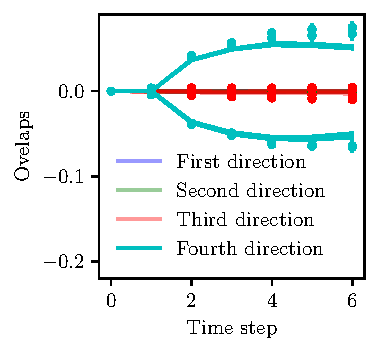
\includegraphics{figs/bad_example} 
    \caption{
    An illustration of a hard, non-even target $f^\star(\vec z) = z_1 z_2 z_3 + \mathrm{He}_3(z_4)$ being learned by a student with $p=4$ hidden units. We can see that, \textit{even when reusing the batch}, the teacher can only learn the direction associated with $z_4$, while keeping a zero overlap otherwise. The continuous lines are from the DMFT numerical integration, the dots are simulations with $d=10000$. In the legend the overlap with the $n$-th direction is the projection of the student weights in the subspace associated with $z_n$. For this figure we have $\sigma = \rm relu$, $n=5d$, $\eta = 0.2$.}
    \label{2402:fig:bad_example}
\end{figure}

We now show the existence of target functions where $E^* \neq OE^*$. Without loss of generality, we assume that the rows of $W^*$ lie along the standard Euclidean basis $\vec{e}_1, \vec{e}_2,\cdots, \vec{e}_k$
\begin{lemma}
    Suppose that $f^*(\vec{z}) = z_1z_2z_3$. Let $\vec{v}^* = \vec{e}_1+\vec{e}_2+\vec{e}_3$. Then $\vec{v}^* \notin E^*$ but $OE^*=U^*$.
\end{lemma}
\begin{proof}
    $\vec{v}^* \notin E^*$ follows directly by noting that $f^*(\vec{z})$ is even-symmetric along $\vec{e}_1-\vec{e}_2$ and $\vec{e}_1-\vec{e}_3$. We further have that a target $f^*$ satisfying $E^*=U^*$ must satisfy $f^*(-\vec{z}) = f^*(\vec{z}) \ \forall \vec{z} \in \R^d$. Therefore, since $f^*(-\vec{z}) = -f^*(\vec{z})$, $f^*$ cannot be even-symmetric along $\vec{e}_1+\vec{e}_2+\vec{e}_3$. 
    Next, we show that $OE^*=U^*$. Since $\vec{e}_1, \vec{e}_2, \vec{e}_3$ span $U^*$, and $f^*$ is symmetric w.r.t permutations of $z_1z_2z_3$, it suffices to show that condition in definition \ref{2402:def:ortho_symmetric_subspace} holds for $\vec{v}^* = \vec{e}_1$. The orthogonal complement $\{\vec{v}^*\}_\perp$ is given by $\operatorname{span}(\vec{e}_2,\vec{e}_3)$. Therefore the transformation $O_2$ defined by $z_2 \rightarrow -z_2$ is a valid orthogonal transformation $O_\perp$ as per definition \ref{2402:def:ortho_symmetric_subspace}. We have:

\begin{align*}
    f^*(O_2 R_{\vec{v}^*}\vec{z}) &= (-z_1)(-z_2)z_3\\
    &= z_1z_2z_3 = f^*(\vec{z}).
\end{align*}
This shows that $\vec{e}_1$ lies in $OE^*$. Similarly, we have by symmetry $\vec{e}_1 \in OE^*$

We present a numerical illustration of another such example in figure \ref{2402:fig:bad_example}.
\end{proof}

One can in-fact construct a family of functions with a direction $\vec{v}^*$, for instance $\vec{v}^* = \vec{e_1}$ lying in $OE^*$ but in general not in $E^*$. To see this, let $f_1$ be a function $\R^d \rightarrow \R$, depending only on projections of $\vec{z}$ along $\{\vec{e}_1\}_\perp$ and let $O_\perp$ by an involutory orthogonal transformation on $\{\vec{e}_1\}_\perp$ i.e an orthogonal transformation satisfying $O^2_\perp = \mathbf{I}$ or equivalently $O_\perp = (O_\perp)^\top$. Now, let $f_2:\R \rightarrow \R$ be an odd function. Then, consider the function:
\begin{equation}
    f^*(\vec{z}) = (f_1(O_\perp \vec{z})-f_(\vec{z}))f_2(z_1).
\end{equation}

We observe that:
\begin{align*}
    f^*(O R_{\vec{e}_1}\vec{z}) &= (f_1(O^2_\perp\vec{z})-f_(O_\perp\vec{z}))f_2(-z_1)\\
    &= (f_1(O_\perp\vec{z})-f_(\vec{z}))f_2(z_1)\\
    &= f^*(\vec{z}),
\end{align*}
where we used that $O^2_\perp = \mathbf{I}$ and $f_2(-z_1)=-f_2(z_1)$. Therefore, for any such function $f^*(\vec{z})$, $\vec{e}_1 \in OE^*$. 

% The above argument can be applied to any $f^*(\vec{z})$


% \subsection{Merging the weights and preactivation stochastic process}



\subsection{Implications for generalization} \label{2402:sec:app:gen_error}
Since the specific guarantees of such results depend on the choice of activation and target functions, we illustrate this for the case of single-index target functions with matching activations:
\begin{corollary}
Consider the setting of a single-index target and student network with matching activations i.e. $\sigma=g^\star$, such that $\sigma$ is a polynomial with finite degree, satisfying the following assumption, $\exists k \in \N$ such that:
\begin{equation}\label{2402:eq:matching}
    \Ea{\sigma^k(z)z}\Ea{D^k\sigma(z)} \neq 0, 
\end{equation},
where $D^k$ denotes the $k_{th}$ derivative.
Let $\hat{\vec{w}}$ be the parameters obtained after two steps of gradient descent with batch size $\cO(d)$ using $\eta$ as in Theorem \ref{2402:thm:main:2step_learning}. Then, almost surely over the initialization $a \sim \mathcal{N}(0,1)$, for any $\epsilon > 0$, there exists a step size $\eta'$ such that online SGD on 
squared loss reaches generalization error $<epsilon$ in time $\cO(d)$. 
\end{corollary}


%\begin{remark}
We verify numerically that the above assumption holds in particular for all odd Hermite polynomials upto order $50$.
    % {\color{red}LZ: Do we want to say "odd" here or "non-even"?}
%\end{remark}
The corollary implies that such target functions can be learned with $\cO(d)$ sample complexity using gradient descent alone, without resorting to specialized algorithms and techniques such as spectral initialization.



\begin{proof}
    Let $\vec{w}^*$ denote the single-direction in the teacher subspace with $\norm{\vec{w}^*}=\sqrt{d}$.
    We note that Equation \eqref{2402:eq:matching} is proportional to the ${k-1}_{th}$ derivative of $\phi(a_j)$ defined in Equation \eqref{2402:eq:phi_def}. Therefore, the condition is sufficient to ensure that $\phi(a_j)$ is not identically zero and the student neuron almost surely develops an overlap along $\vec{w}^*$.
    The result then follows from
    Proposition 2.1 in \citep{arous2021online}, which proves that upon weak recovery i.e a non-zero overlap the target direction $\vec{v}^*$, online SGD on a differentiable activation with polynomially bounded derivatives converges to strong recovery Concretely, for any starting non-zero overlap $\theta > 0$, for any $\epsilon' > 0$, there exists $C_{\epsilon',\theta}$ and small-enough step-size such that online SGD with time $C_{\epsilon',\theta} d$ achieves overlap $1-\epsilon'$ along $\vec{w}^*$
    Due to the matching activations, this suffices to obtain arbitrary generalization error.
    \end{proof}



\section{General Multi-Pass Schemes}\label{2402:sec:app:repeat}


\begin{figure*}
    \centering
    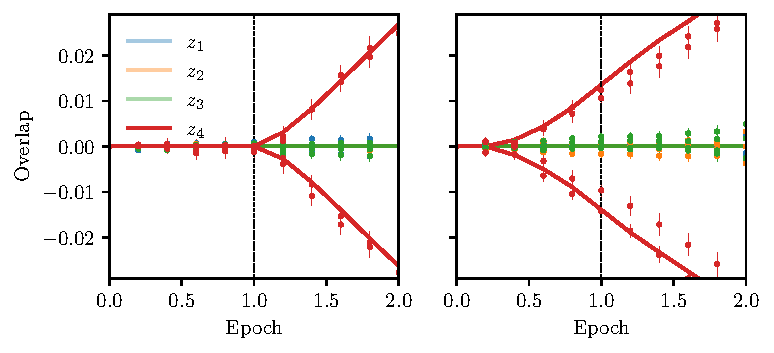
\includegraphics{figs/overlaps_batch}
    \caption{Comparison of theory and experiments for Gradient Descent on the target $z_1z_2z_3 + \mathrm{He}_3(z_4)$. Each gradient step uses a mini-batche of $n/5$ samples. On the {\bf left} we use the data sequentially, on the {\bf right} we sample the batch from the dataset with replacement. The continuous lines are from the DMFT numerical integration, the dots are simulations with $d=10000$ averaged over $32$ realisations. In the legend the overlap with the $n$-th direction is the projection of the student weights in the subspace associated with $z_n$. For this figure we have $\sigma = \rm relu$, $n=5d$, $\eta = 0.2$.}
    \label{2402:fig:overlaps_batch}
\end{figure*}

\subsection{Sketch of Proof for Extending Theorem \ref{2402:thm:main:2step_learning} to Cycling over Epochs}
Let $\vec{Z}^1,\cdots, \vec{Z}^n_e$ denote $n_e$ independent minibatches of size $n_b$ such that $\frac{n_b}{d} = \mathcal{O}(1)$ with $n_e$ being finite. The effective dynamics for a finite number of epochs can be obtained by noting that Theorem 3.2 in \cite{gerbelot2022rigorous} allows generalizing Theorem \ref{2402:thm:Cedric_theorem} to dynamics of the form:
 \begin{align}
        W^{(t+1)} =  W^{(t)} - \eta \lambda W^{(t)} -  \sum_{i=1}^{n_e}\eta \frac{1}{\sqrt{d}}\sum_{\nu=1}^{n_b} F^t_i\left(\frac{ W^{(t)}\vec z^i_\nu} {\sqrt{d}}\right) (\vec z^i_\nu)^\top.
    \end{align}
The above form of the dynamics allows a different update to be utilized for data corresponding to different blocks  $\vec{Z}^1,\cdots, \vec{Z}^n_e$. In particular, setting $F^t_i$ to $0$ whenever $t\mod i \neq 0$  and $\nabla_{\boldsymbol{h}} \mathcal{L}$ otherwise, results in a cycling schedule over the mini-batches $\vec{Z}^1,\cdots, \vec{Z}^n_e$. Subsequently, one can show that the update from $\vec{Z}^i$ in the first-epoch leads to the hidden-progress effect on $M^{t}$ when the model re-uses $\vec{Z}^i$ in the second epoch.

We believe a similar result would hold for $n_b = \mathcal{O}(1)$ samples in the minibatch, as displayed in Figure \ref{2402:fig:overlaps_minibatch}


\begin{figure}
    \centering
    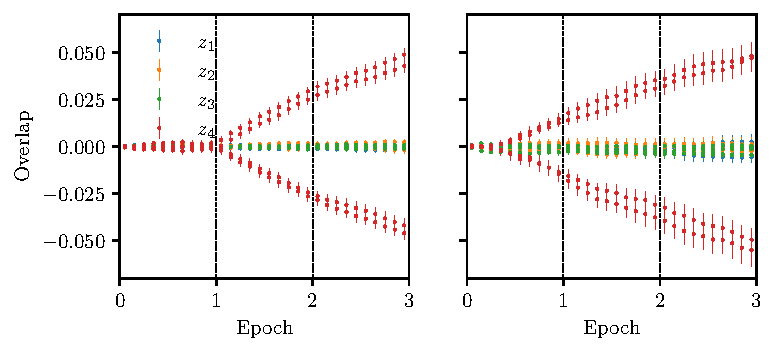
\includegraphics{figs/overlaps_minibatch}
    \caption{Experiments for Gradient Descent on the target $z_1z_2z_3 + \mathrm{He}_3(z_4)$. We use minibatches with $1$ sample each. On the {\bf left} we use the data sequentially, on the {\bf right} we sample the data point from the dataset with replacement. The dots are simulations with $d=10000$ averaged over $32$ realisations. In the legend the overlap with the $n$-th direction denotes the projection of the student weights in the subspace associated with $z_n$. For this figure we have $\sigma = \rm relu$, $n=5d$, $\eta = 0.2$.}
    \label{2402:fig:overlaps_minibatch}
\end{figure}
